\begin{ledgroupsized}[r]{120mm}
\footnotesize 
\pstart 
\noindent\textbf{\"{U}berlieferung:}
\pend
\end{ledgroupsized}
\begin{ledgroupsized}[r]{114mm}
\footnotesize 
\pstart \parindent -6mm
\makebox[6mm][l]{\textit{L}}Aufzeichnung:
LH XXXV 10, 9 Bl. 3-4. 1 Bog. 2\textsuperscript{o}.
\nicefrac{1}{2} Sp. auf Bl. 3~r\textsuperscript{o} links oben.
Der übrige Text auf Bl. 3~r\textsuperscript{o} gehört zu N.~28\textsubscript{5}. % = LH035,10,9 Bl. 3r_2 = Regula de vi ponderis
Der Bog. überliefert ferner N.~28\textsubscript{1}, % = LH035,10,9 Bl. 3v_1 = Règle pour calculer la force d'une machine 1
N.~28\textsubscript{2} % = LH035,10,9 Bl. 3v_2 = Règle pour calculer la force d'une machine 2
und N.~28\textsubscript{6}.% = LH035,10,9 Bl. 4 = De determinatione machinae virium
\\%
Cc 2, Nr. 1191 (tlw.)
\pend
\end{ledgroupsized}
%
\vspace*{5mm}
\begin{ledgroup}
\footnotesize 
\pstart
\noindent\footnotesize{\textbf{Datierungsgr\"{u}nde}: Das vorliegende Stück befindet sich zusammen mit Unterstücken von N. 28 %
% = LH035,10,9 Bl. 1-4 = Règle pour calculer la force d'une machine
auf einem Bogen und dürfte daher zeitnah zu diesen letzteren entstanden sein.
Die Datierung von % = LH035,10,9 Bl. 1-4 = Règle pour calculer la force d'une machine
N.~28~--~zweite Hälfte 1674 bis Anfang 1675 -- wird demgemäß auch für das vorliegende Stück übernommen.}
\pend
\end{ledgroup}
%
\vspace*{8mm}
\pstart 
\normalsize
\begin{wrapfigure}[13]{l}{0.38\textwidth}  
\vspace{-5mm}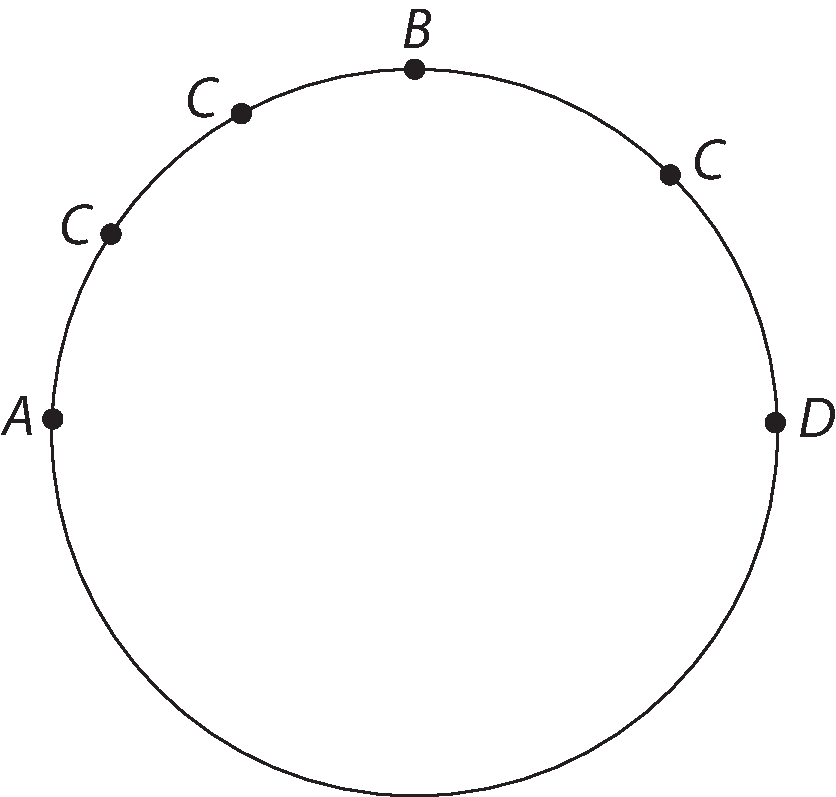
\includegraphics[trim = 0mm -3mm -4mm 0mm, clip, width=0.38\textwidth]{images/lh0351009_003r-d1.pdf}\\
\centering[\textit{Fig. 1}]
\end{wrapfigure}
\noindent%
% [3~r\textsuperscript{o}]
[3~r\textsuperscript{o}] Experiundum est, an Magnes\protect\index{Sachverzeichnis}{magnes} habeat sphaeram activitatis\protect\index{Sachverzeichnis}{sphaera activitatis} determinatam, id est, pone Magnetem elevare posse certum ferri\protect\index{Sachverzeichnis}{ferrum} pondus\protect\index{Sachverzeichnis}{pondus} ex distantia data; ita ut aucta distantia elevare amplius non possit; quaeritur an aucta distantia omnino non agat in ferrum\protect\index{Sachverzeichnis}{ferrum} illud. Hoc ita experiri licet: Pone ferrum\protect\index{Sachverzeichnis}{ferrum} illud in fundo vasis\protect\index{Sachverzeichnis}{vas} aqua\protect\index{Sachverzeichnis}{aqua} pleni esse; distantia a magnete\protect\index{Sachverzeichnis}{magnes} superposito, majore paulo quam ut ab eo attrahi possit. Jam infigamus illud ferrum\protect\index{Sachverzeichnis}{ferrum} rei cuidam levi ut suberi\protect\index{Sachverzeichnis}{suber}; ita tamen ut pondus\protect\index{Sachverzeichnis}{pondus} ferri\protect\index{Sachverzeichnis}{ferrum} praeponderet levitati suberis\protect\index{Sachverzeichnis}{suber}; id est ut maneat in fundo: Experiundum erit admoto magnete, an frustum illud ex ferro\protect\index{Sachverzeichnis}{ferrum} et subere\protect\index{Sachverzeichnis}{suber} elevare possit; nam si elevat; sequitur sphaeram illam activitatis\protect\index{Sachverzeichnis}{sphaera activitatis} non fuisse determinatam; sed magnetem\protect\index{Sachverzeichnis}{magnes} egisse in ferrum\protect\index{Sachverzeichnis}{ferrum} etsi non satis fortiter, quod nunc apparet; quoniam levius redditum attolit. Sin minus patet magnetem habere sphaeram activitatis\protect\index{Sachverzeichnis}{sphaera activitatis} determinatam; ultra quam omnino non agat.
\pend
\pstart
Idem sic quoque facilius indagari potest; examinando an sit distantia quaedam assignabilis; ex qua magnes\protect\index{Sachverzeichnis}{magnes} frustum ferri\protect\index{Sachverzeichnis}{ferrum} parvum elevet, majus quod ex minore elevaret, non \edtext{elevaret. 
Hinc patebit an magnes eadem vi agat in magna parva distantia.}{\lemma{\hspace{1.8mm}27-S. 51.1}\killnumber\Bfootnote{elevaret.\ \textbar\ Hinc [...] distantia. \textit{erg.}\ \textbar\ \textit{(1)}\ Si duo \textit{(2)}\ Si sit \textit{L}}} \pend
\newpage
\pstart
Si sit pila\protect\index{Sachverzeichnis}{pila} ferrea, et duobus magnetibus\protect\index{Sachverzeichnis}{magnes} in oppositis punctis $\displaystyle A. D$, opposito modo fricetur, ponendo magnetes esse aequales, destruetur effectus mutuo. Jam examinandum est, quid fiat, si fricetur simul in $\displaystyle A$ et $\displaystyle C$ pro varia anguli ratione.
\pend
\pstart
Experiendum an eundem effectum faciat annulus\protect\index{Sachverzeichnis}{annulus} ferreus, quem pila\protect\index{Sachverzeichnis}{pila} aut acus\protect\index{Sachverzeichnis}{acus}: idem quae aliae a figuris varietates. Experiendum an mutatio oriatur, certis partibus in magnete\protect\index{Sachverzeichnis}{magnes} \edtext{aut pila\protect\index{Sachverzeichnis}{pila}}{\lemma{aut pila}\Bfootnote{\textit{erg. L}}}
igne mutilibus redditis, v.g. aequatore\protect\index{Sachverzeichnis}{aequator}; et aliis; item quid fiat uno polo\protect\index{Sachverzeichnis}{polus} ignito, altero \edtext{relicto.}{\lemma{altero}\Bfootnote{\textit{(1)}\ destructo \textit{(2)}\ relicto \textit{L}}}
\pend
\pstart
De ratione faciendi compassum\protect\index{Sachverzeichnis}{compassus} nauticum maximum ad minuta usque secunda divisum. Acus\protect\index{Sachverzeichnis}{acus} magneticae in extremitate $\displaystyle M.$
\pend
\pstart
De modo inclinationem\protect\index{Sachverzeichnis}{inclinatio} et declinationem\protect\index{Sachverzeichnis}{declinatio} ad regulam revocandi, in terra\protect\index{Sachverzeichnis}{terra}: per $\displaystyle P$ parallelos et meridianos.
\pend
\pstart
Magnetis\protect\index{Sachverzeichnis}{magnes} vis attractiva\protect\index{Sachverzeichnis}{vis attractiva} $c+g+h$, pondus\protect\index{Sachverzeichnis}{pondus} \edtext{[pilulae]}{\lemma{pilylae}\Bfootnote{\textit{L \"{a}ndert Hrsg.}}} \edtext{ferro\protect\index{Sachverzeichnis}{ferrum} gravis}{\lemma{ferro}\Bfootnote{\textit{(1)}\ imbuit \textit{(2)}\ gravis \textit{L}}} $g+h$. $\displaystyle h$ pondus\protect\index{Sachverzeichnis}{pondus} aquae\protect\index{Sachverzeichnis}{aqua} paris spatii[,] $\displaystyle c+g+h+d$ 
pondus\protect\index{Sachverzeichnis}{pondus} ipsius magnetis\protect\index{Sachverzeichnis}{magnes}[,] ex centro $\displaystyle E,$ radio $\displaystyle EC.$
Hactenus figura data, fiat nova.
\pend 
